
\section{Introduction}
Within systems neuroscience, significant efforts have been made to elucidate and analyze and the neural representation of objects and their categories. In humans, visual object recognition is generally accomplished rapidly and with minimal conscious effort, however this belies the true complexity of the task. And, while a practical mechanistic understanding of object recognition may currently fall beyond our reach, significant progress has been made in investigating the spatio-temporal dynamics of the process. 

Electroencephalography (EEG) has played an important role in these advances. Owing to its high temporal resolution, EEG allows us to investigate the rapid transformations of neural activity that underlie perception. In particular, EEG decoding studies have proven a popular paradigm in this area of research. In a decoding study, stimuli are presented to subjects, and contemporaneous neural responses to these stimuli are recorded. A decoding model is then trained on these responses to discriminate the property of interest. Frameworks such as representational similarity analysis (RSA) can be used to investigate organization of neural responses by comparing the similarity of patterns learned by a decoding model across conditions~\cite{Kriegeskorte:2008}. However, due to the complexity of the process, the noise inherent to the recording modality, and the resource intensive nature of data acquisition, EEG decoding presents substantial challenges.  

In this work, we attempt to replicate a target study which sought to extend this line of inquiry by introducing a novel classification-based RSA method~\cite{Kaneshiro:2015}. Rather than deriving representational dissimilarity matrices (RDMs) from pairwise classification accuracies, as done in prior work, the authors employed confusion matrices from multi-class classifiers applied to single-trial EEG data. This method was intended to determine whether emergent properties arising from the simultaneous consideration of multiple classes would yield a richer and more informative representational structure than traditional pairwise approaches. Additionally, the study aimed to localize the spatial and temporal components of EEG activity that contributed most strongly to category-level and exemplar-level distinctions. The reported findings appeared to support the effectiveness of this approach. In our replication attempt, we found that while it was possible to reproduce the reported results by following the methodology described in the target study, the validity of that methodology was suspect. In particular, a cross-validation method employed by several publications, including the target study, was shown to be confounded by the repetition of stimuli, resulting in a substantial overestimation of decoding accuracy. However, the extent to which this confound affects analyses performed in the target study has not yet been established. A further examination of the procedures in the target study uncovered two additional methodological issues: (i) principal components derived from the entire feature matrix were used to reduce dimensionality, enabling test set leakage, and (ii) the dissimilarity metric used to compute the RDMs is invalid, as it violates both non-negativity and unit self-similarity. In aggregate, we found these issues severely undermine the evidential basis of the reported findings, and warranted further analysis.

In the following, we discuss our replication attempt, our analysis of the methodological issues affecting the target study, and the broader implications of our findings for classification-based RSA in EEG research.

\section{Materials and Methods}
\subsection{Data collection and processing in the target study}

The Stanford University Dataset (SUD) consists of preprocessed EEG recordings from 10 subjects, obtained while they viewed 72 images evenly distributed across 6 categories. To reduce the impact of trial-to-trial variation, each stimulus was presented 72 times to each subject, for a total of 5,184 trials per subject. The stimuli were recorded in six blocks of 864 trials each, over two sessions. In each block, all stimuli appeared 12 times, in a randomized order. Each stimulus was presented for 500~ms, followed by a 750~ms inter-stimulus interval, during which a gray background was displayed. The data was recorded using a 128-channel EEG system with a sampling rate of 1~kHz. The EEG signals were then preprocessed using a high-pass fourth-order Butterworth filter to attenuate frequencies below 1~Hz, and a low-pass Chebyshev Type I filter to attenuate frequencies above 25~Hz. The data was then subsampled to 62.5~Hz to reduce the computational cost of the analysis. Ocular artifacts were removed using the Bell-Sejnowski Infomax independent-component-analysis algorithm~\cite{Bell-Sejnowski:1995}.  The 4 channels used to detect ocular artifacts were removed, and the remaining channels were converted to average reference. Finally, epochs of 496~ms post-stimulus response, time-locked to the onset of the stimulus, were extracted from the data. As a result, each trial is represented as a 124$\times$32 feature matrix, where the first dimension represents the 124 channels which were retained, and the second dimension represents the 32 time points of post-stimulus response for each trial. See Fig.~\ref{fig:sud-category-structure} for a visualization of the category structure of the SUD. 

\begin{SCfigure}
    \centering
    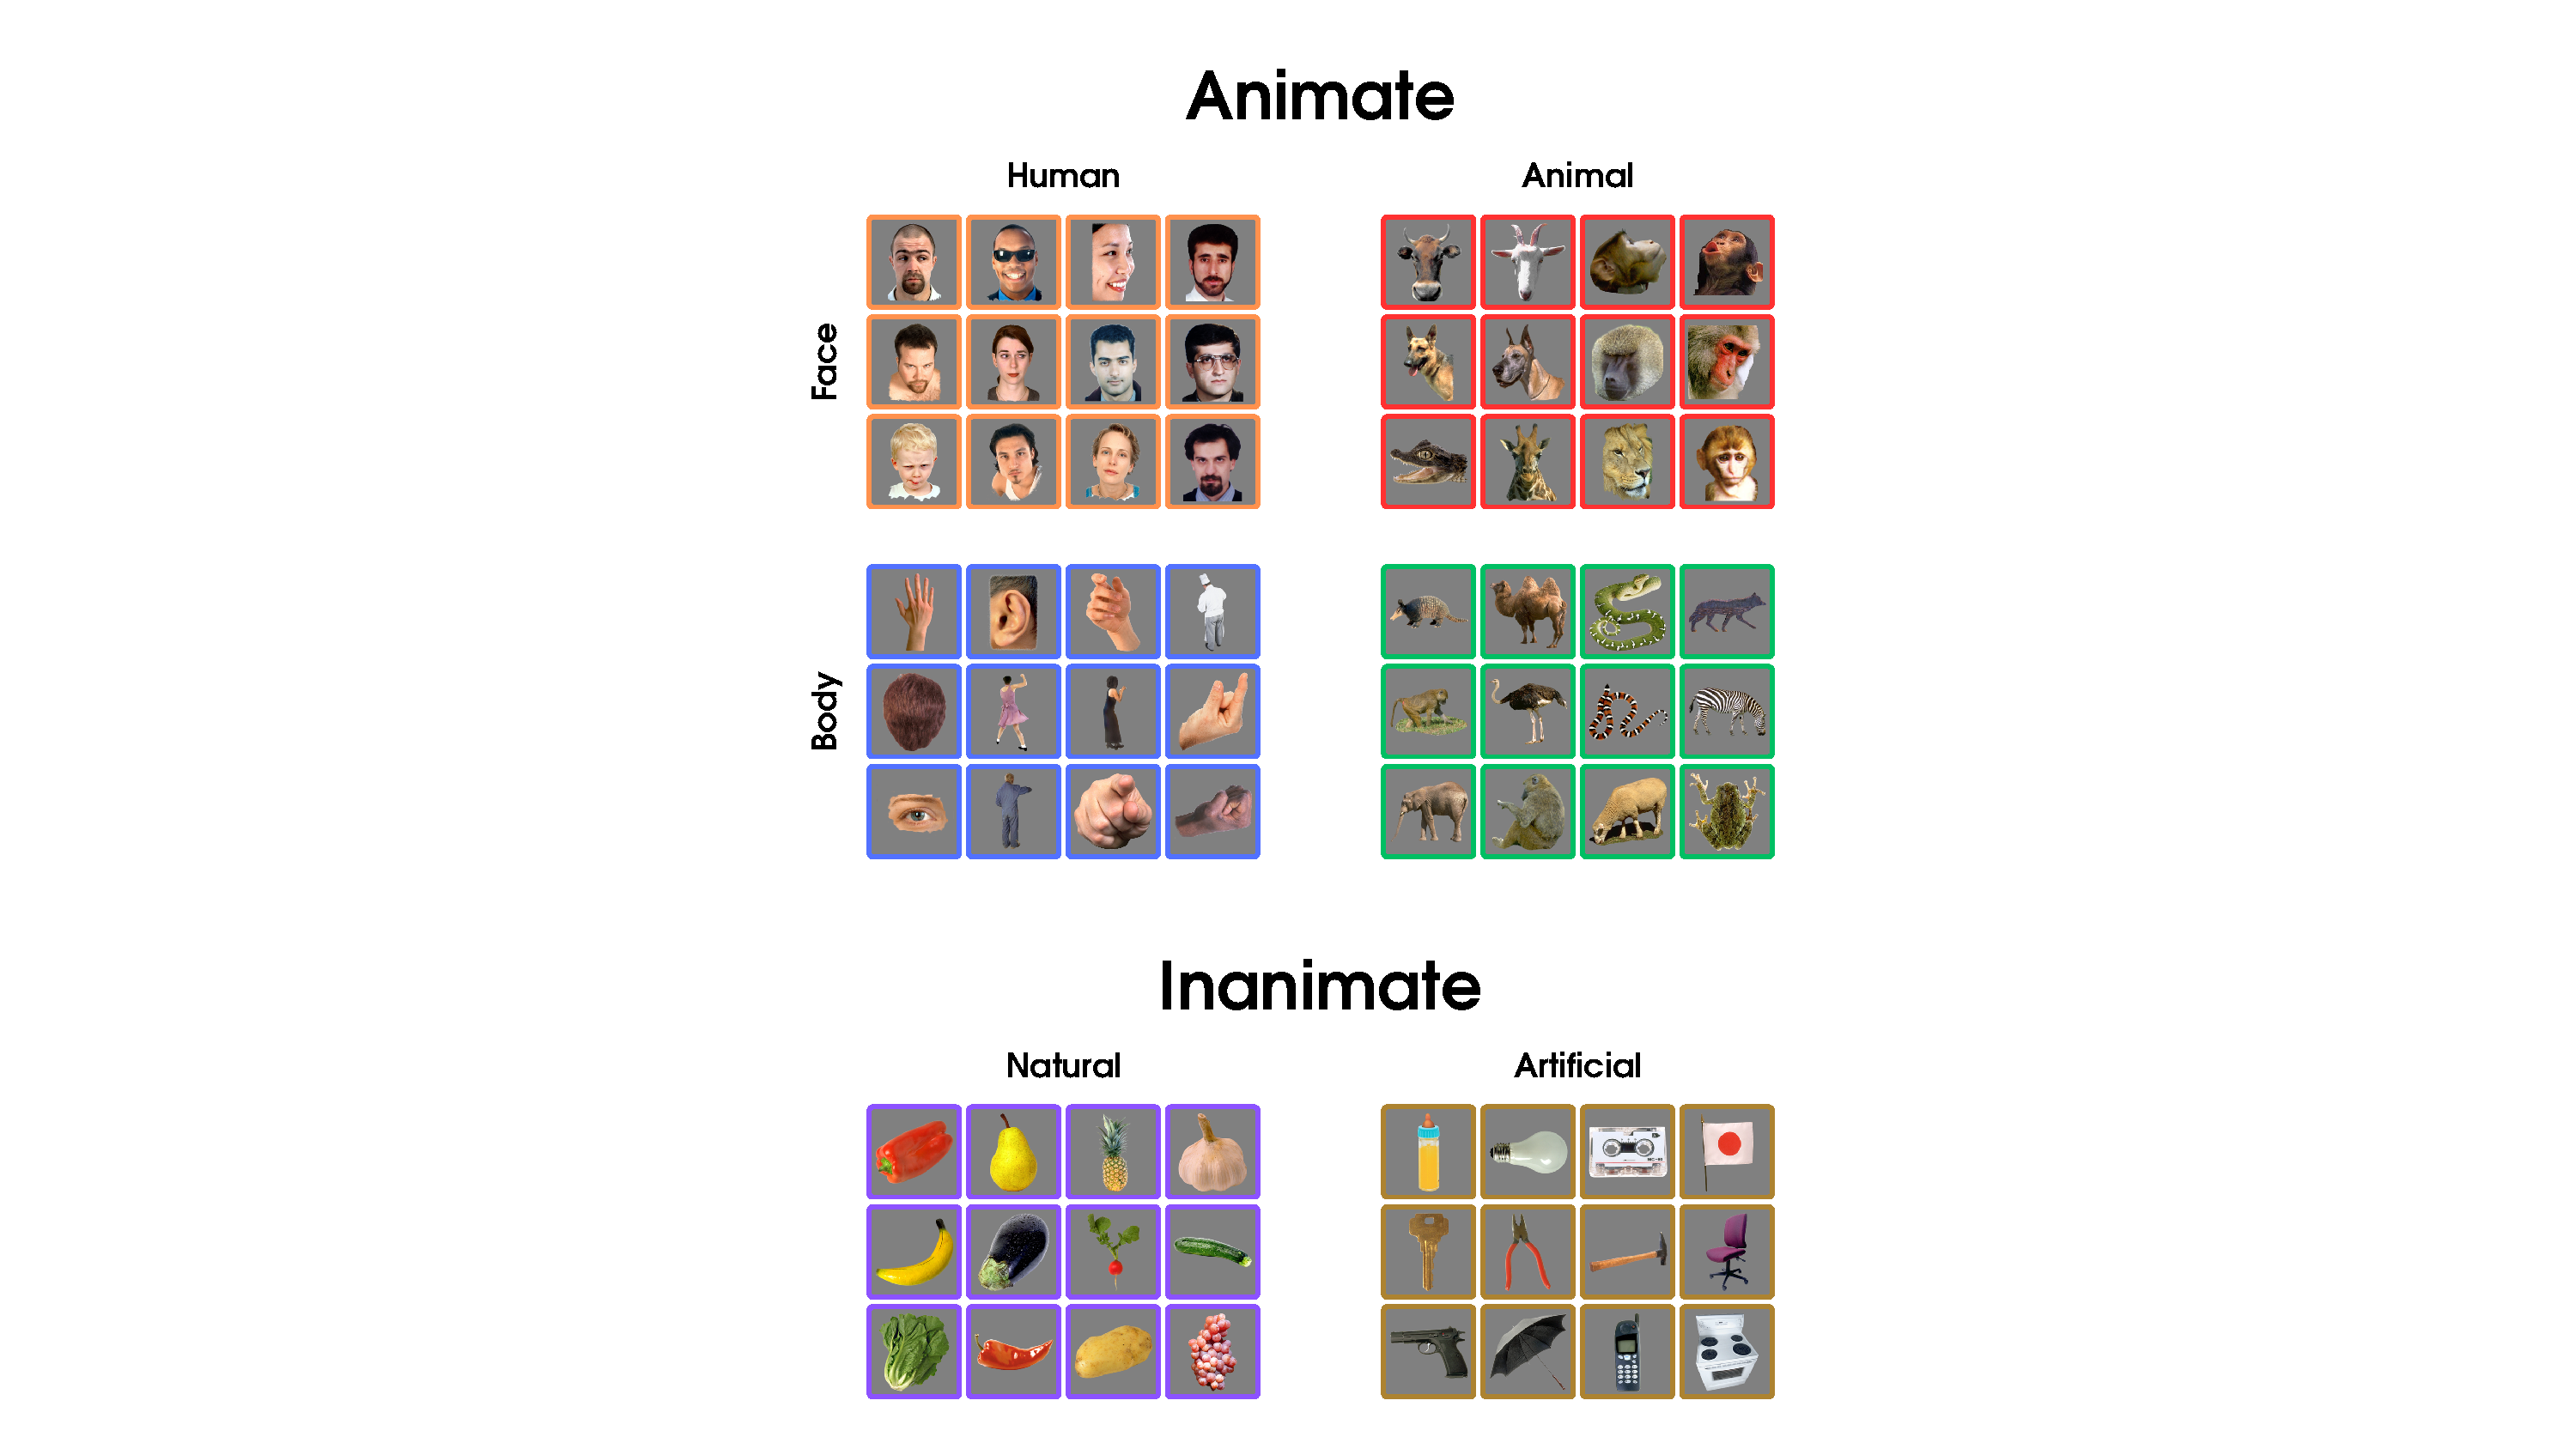
\includegraphics[width=7.5cm, trim={16cm, 0cm, 15cm, 1.0cm}, clip]{sudb_stimuli_by_category}
  \caption{\textbf{The category and structure of the SUD stimulus set.} The stimulus set used in the SUD is composed of 72 images of natural objects. In the original category structure of the SUD (left), these stimuli are evenly distributed across six categories: Human Body (HB), Human Face (HF), Animal Body (AB), Animal Face (AF), Fruit/Vegetable (FV), and Inanimate Object (IO). These can be further grouped into Animate and Inanimate supercategories.\vspace{15em}}
  \label{fig:sud-category-structure}
\end{SCfigure}

\subsection{Analyses in the target study}

In the target study, the primary analyses comprise five decoding tasks: two at the concept level (category decoding and human-face vs. artificial-object decoding) and three at the stimulus level (exemplar decoding, human-face decoding, and artificial-object decoding). Four variants of each task were performed to isolate spatio-temporal dynamics. In the baseline task, decoding models were trained and evaluated using signals from all electrodes across all timepoints. To isolate spatial contributions, models were trained to decode the signals of individual electrodes. Similarly, to isolate the separability of classes over time, another task was performed in which models were trained on windows of consecutive time points. Finally, to assess spatio-temporal variability, a fourth task was performed by training models on temporal windows from individual electrodes.

 To reduce the dimensionality of the data, singular-value decomposition (SVD) was performed. To reduce the computational expense of the analyses, SVD was evaluated using the entire feature matrix for each subject. For each task, nested cross-validation was performed. The inner cross-validation folds were used to select the optimal number of principal components to use in dimensionality reduction, while the outer fold is used to estimate decoding accuracy and analyze model predictions. Subsequently, the confusion matrices of model predictions are used to investigate the representational similarity of different conditions in the target task. This is achieved by calculating a dissimilarity measure $D$ from the confusion matrices using equation~\ref{eqn:dissimilarity-measure}.

\begin{equation}
    D_{ij} = 1 - \sqrt{\frac{C_{ij}}{C_{jj}}\cdot \frac{C_{ji}}{C_{ii}}} \label{eqn:dissimilarity-measure}
\end{equation}

The resulting dissimilarity measure is then used to visualize the representational space of the target property using multidimensional scaling (MDS). Additionally, hierarchical clustering was performed using an unweighted pair grouping method with averaging (UPGMA) and the results were visualized as dendrograms. 

\section{Our analysis pipeline}
As mentioned previously, the methodology employed by the target study strategy suffers from three major issues. Firstly, as multiple responses to each stimulus were recorded, the test data consists of responses to stimuli already used to train models, which inflates estimates of model accuracy in the category decoding and human face vs artificial object decoding tasks. Secondly, by using the SVD of the entire feature matrix in dimensionality reduction, features of the test set may leak to the training set further inflating accuracy. Thirdly, the dissimilarity measure used does not satisfy the requirements of a dissimilarity measure. In particular, if a class is misclassified more often than it is correctly classified, then the measure returns negative values which are outside the defined range of a dissimilarity measure. 

To facilitate a robust replication, and determine the extent to which these issues limit the reproducibility of the target study we consequently made the following modifications. First, in the case of the category decoding and human face vs artificial object decoding tasks, we employed the paired cross-validation strategy from~\textcite{Kilgallen:2025} to investigate the extent to which the repetition of stimuli affects primary claims of the target study. However, the target study used 10-fold cross validation while the stimulus set has 12 stimuli per category. Consequently, to produce directly comparable results with and without stimulus repetition, all 12-fold cross validation was applied in all experiments. Secondly, in all experiments we perform dimensionality reduction using only the principal components of the training data. And lastly, we restricted the range of the dissimilarity measure to non-negative real numbers by clipping all negative values to zero.

\section{Results}

\subsection{Category-level classifications}
\begin{figure}
    \begin{minipage}[b]{0.32\columnwidth}
        \includegraphics[width=\columnwidth]{SUDB_full_response_category_decoding/LDA/all_electrodes/all_timepoints/unconfounded_test/confusion_matrix}
    \end{minipage}
    \begin{minipage}[b]{0.32\columnwidth}
        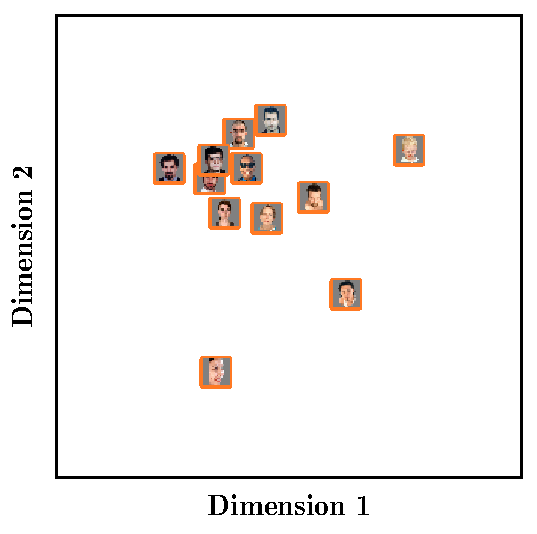
\includegraphics[width=\columnwidth]{SUDB_full_response_category_decoding/LDA/all_electrodes/all_timepoints/unconfounded_test/MDS}
    \end{minipage}
    \begin{minipage}[b]{0.32\columnwidth}
        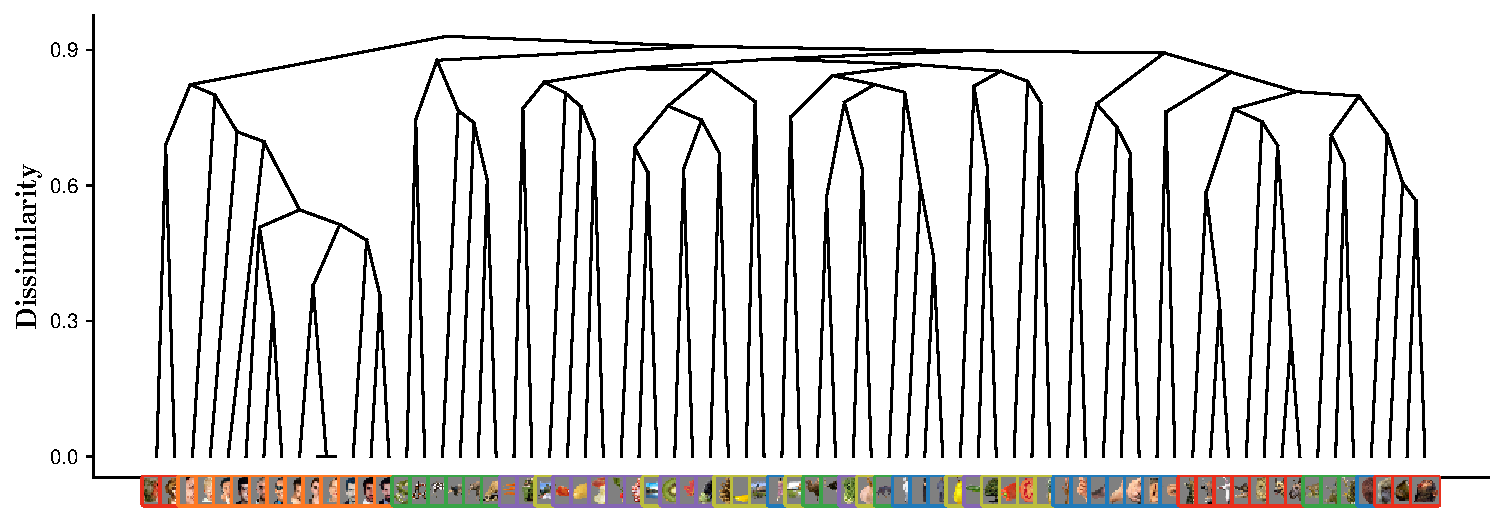
\includegraphics[width=\columnwidth]{SUDB_full_response_category_decoding/LDA/all_electrodes/all_timepoints/unconfounded_test/dendrogram.pdf}
    \end{minipage}
    \caption{\textbf{Category-level classification results.}}
\end{figure}

\begin{SCfigure}
    \centering
    \includegraphics[width=0.5\columnwidth]{SUDB_single_electrode_category_decoding/LDA/all_timepoints/unconfounded_test/topomap.pdf}
    \caption{\textbf{Topographic map of category-level classifier accuracies for individual electrodes.}\vspace{15em}}
\end{SCfigure}
\begin{figure}
    \centering
        \includegraphics[width=\columnwidth]{SUDB_temporal_window_category_decoding/LDA/all_electrodes/unconfounded_test/time_course}
        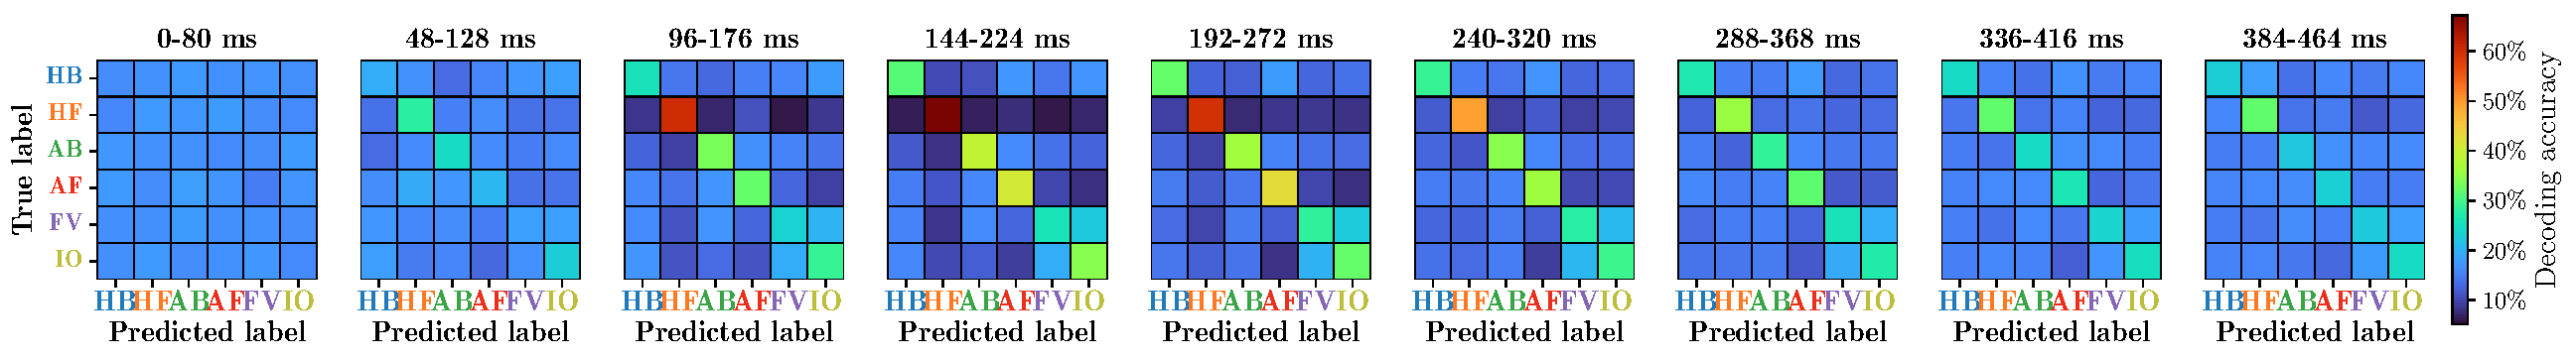
\includegraphics[width=\columnwidth]{SUDB_temporal_window_category_decoding/LDA/all_electrodes/unconfounded_test/confusion_matrices}
        \includegraphics[width=0.90\columnwidth]{SUDB_temporal_window_category_decoding/LDA/all_electrodes/unconfounded_test/mds}
        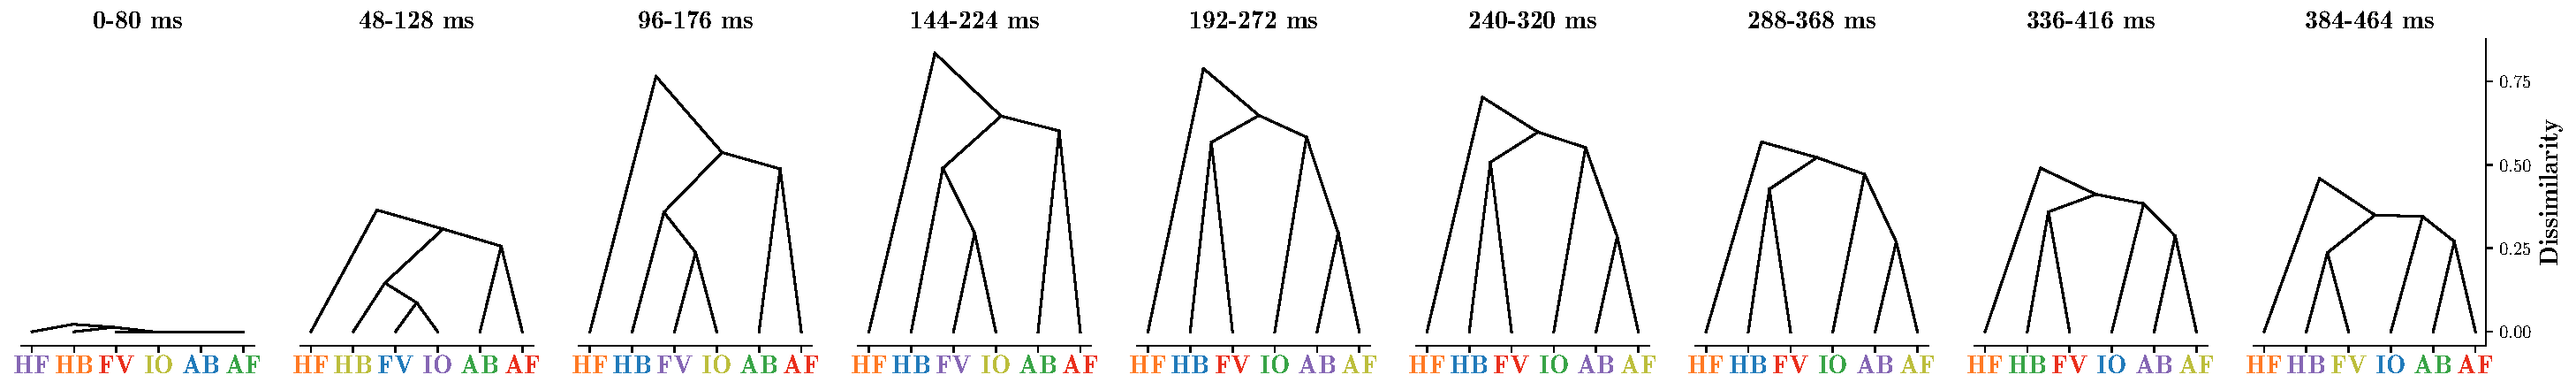
\includegraphics[width=0.95\columnwidth]{SUDB_temporal_window_category_decoding/LDA/all_electrodes/unconfounded_test/dendrograms}
    \caption{\textbf{Temporally resolved category-level classification results.}}
\end{figure}
\begin{figure}
    \centering
        \includegraphics[width=\columnwidth]{SUDB_single_electrode_temporal_window_category_decoding/LDA/unconfounded_test/topomaps}
    \caption{\textbf{Temporally resolved rate maps for single-electrode category-level classifications.}}
\end{figure}

\subsection{Exemplar-level classifications}
\begin{figure}
    \centering
        \includegraphics[width=\columnwidth]{SUDB_full_response_exemplar_decoding/LDA/all_electrodes/all_timepoints/test/confusion_matrix}
    \caption{\textbf{Exemplar-level classification results.}}
\end{figure}
\begin{figure}
    \centering
        \includegraphics[width=\columnwidth]{SUDB_full_response_exemplar_decoding/LDA/all_electrodes/all_timepoints/test/mds}
    \caption{\textbf{Multidimensional scaling plots for exemplar-level classification.}}
\end{figure}

\begin{figure}
    \centering
        \includegraphics[width=\columnwidth]{SUDB_temporal_window_exemplar_decoding/LDA/all_electrodes/test/time_course}
    \caption{\textbf{Temporally resolved exemplar-level classification results.}}
\end{figure}

\subsection{Within-Category Classifications}
\begin{figure}
    \begin{minipage}[b]{0.32\columnwidth}
        \includegraphics[width=\columnwidth]{SUDB_full_response_human_face_decoding/LDA/all_electrodes/all_timepoints/test/confusion_matrix}
    \end{minipage}
    \begin{minipage}[b]{0.32\columnwidth}
        \includegraphics[width=\columnwidth]{SUDB_single_electrode_human_face_decoding/LDA/all_timepoints/test/topomap}
    \end{minipage}
    \begin{minipage}[b]{0.32\columnwidth}
        \includegraphics[width=\columnwidth]{SUDB_temporal_window_human_face_decoding/LDA/all_electrodes/test/time_course}
    \end{minipage}
    \begin{minipage}{\columnwidth}
        \includegraphics[width=\columnwidth]{SUDB_single_electrode_temporal_window_human_face_decoding/LDA/test/topomaps}
    \end{minipage}
    \caption{\textbf{Face classification results.}}
\end{figure}

\begin{figure}
    \begin{minipage}[b]{0.32\columnwidth}
        \includegraphics[width=\columnwidth]{SUDB_full_response_artificial_object_decoding/LDA/all_electrodes/all_timepoints/test/confusion_matrix}
    \end{minipage}
    \begin{minipage}[b]{0.32\columnwidth}
        \includegraphics[width=\columnwidth]{SUDB_single_electrode_artificial_object_decoding/LDA/all_timepoints/test/topomap}
    \end{minipage}
    \begin{minipage}[b]{0.32\columnwidth}
        \includegraphics[width=\columnwidth]{SUDB_temporal_window_artificial_object_decoding/LDA/all_electrodes/test/time_course}
    \end{minipage}
    \begin{minipage}{\columnwidth}
        \includegraphics[width=\columnwidth]{SUDB_single_electrode_temporal_window_artificial_object_decoding/LDA/test/topomaps}
    \end{minipage}
    \caption{\textbf{Object classification results.}}
\end{figure}

\begin{figure}
    \begin{minipage}[b]{0.32\columnwidth}
        \includegraphics[width=\columnwidth]{SUDB_full_response_human_face_vs_artificial_object_decoding/LDA/all_electrodes/all_timepoints/unconfounded_test/confusion_matrix}
    \end{minipage}
    \begin{minipage}[b]{0.32\columnwidth}
        \includegraphics[width=\columnwidth]{SUDB_single_electrode_human_face_vs_artificial_object_decoding/LDA/all_timepoints/unconfounded_test/topomap}
    \end{minipage}
    \begin{minipage}[b]{0.32\columnwidth}
        \includegraphics[width=\columnwidth]{SUDB_temporal_window_human_face_vs_artificial_object_decoding/LDA/all_electrodes/unconfounded_test/time_course}
    \end{minipage}
    \begin{minipage}{\columnwidth}
        \includegraphics[width=\columnwidth]{SUDB_single_electrode_temporal_window_human_face_vs_artificial_object_decoding/LDA/unconfounded_test/topomaps}
    \end{minipage}
    \caption{\textbf{Face vs Object classification results.}}
\end{figure}

\section{Discussion}
\subsection{Understanding the representational structure of object categories}
\subsection{Re-evaluating the temporal dynamics of object recognition}
\subsection{Re-assesssing spatial dynamics of object recognition}

\section{Conclusion}